%-----------------------------------------------------------------------------
%
%               Template for sigplanconf LaTeX Class
%
% Name:         sigplanconf-template.tex
%
% Purpose:      A template for sigplanconf.cls, which is a LaTeX 2e class
%               file for SIGPLAN conference proceedings.
%
% Guide:        Refer to "Author's Guide to the ACM SIGPLAN Class,"
%               sigplanconf-guide.pdf
%
% Author:       Paul C. Anagnostopoulos
%               Windfall Software
%               978 371-2316
%               paul@windfall.com
%
% Created:      15 February 2005
%
%-----------------------------------------------------------------------------


\documentclass[10pt,reprint]{socc14}

\usepackage{amsmath}
\usepackage{color}
\usepackage{mathptmx}
\usepackage{graphicx, subfigure}
\usepackage{url}
\usepackage{comment}
\usepackage{titlesec}

%\hyphenation{diver-sifi-cation}

\begin{document}

\special{papersize=8.5in,11in}
\setlength{\pdfpageheight}{\paperheight}
\setlength{\pdfpagewidth}{\paperwidth}

\conferenceinfo{Submission to SoCC '15}{August, 2015, Kohala Coast, HI, USA} 
\copyrightyear{2015} 
\copyrightdata{978-1-nnnn-nnnn-n/yy/mm} 
\doi{nnnnnnn.nnnnnnn}

% Uncomment one of the following two, if you are not going for the 
% traditional copyright transfer agreement.

%\exclusivelicense                % ACM gets exclusive license to publish, 
                                  % you retain copyright

%\permissiontopublish             % ACM gets nonexclusive license to publish
                                  % (paid open-access papers, 
                                  % short abstracts)

%\titlebanner{banner above paper title}        % These are ignored unless
%\preprintfooter{short description of paper}   % 'preprint' option specified.

\title{Scalable Overlay for Data Aggregation in Datacenters}
%\subtitle{Subtitle text, if any}

\authorinfo{Haoyan Geng}
           {Cornell University}
           {geng@cs.cornell.edu}
\authorinfo{Robbert van Renesse}
           {Cornell University}
           {rvr@cs.cornell.edu}

\maketitle

\subsection*{Abstract}



\section{Introduction}\label{sec:intro}

Data aggregation is an integral service for many cloud-based applications.
Such service constantly collects data generated from a large number of sources,
before performing analysis or making decisions.  An example is distributed
messaging service, where a message bus collects messages from many publishers.
Large scale monitoring systems also have similar requirements.  A cluster
management utility would collect performance numbers periodically from all the
machines within a datacenter.  Similar data aggregation occurs in intelligent
sensor networks such as smart power grid and smart home systems.

Formally, given a large number of senders and a single receiver, this paper
addresses the problem of optimizing throughput at the receiver.  This problem
resembles a reversed version of the multicast problem.  In particular, like a
typical tree-based multicast systems, a straightforward solution is to build a
tree structure among the nodes, with the receiver be the root.  Within the tree,
each node forwards messages generated by itself and all other nodes in its
subtree upwards, all the way to the root.

As in tree-based multicast, however, a major limitation with this simple
approach is load imbalance.  Since a node receives and forwards messages from
all the nodes below itself, the load on non-leaf/internal nodes is much higher
than that on leaf nodes of the tree.  In fact, nodes closer to the root receive
higher load, and the maximum throughput of the whole system is bounded by
available bandwidth at the root.

An important difference between the data aggregation problem and multicast is
that in data aggregation, each node generates its own data independently, rather
than forwarding the same data from a unique sender as in multicast.  This
provides the possibility for internal nodes to reduce the load imbalance by
compress the data before forwarding.

This paper presents a system that optimizes data aggregation throughput.  The
key idea in our system is to insert \emph{artificial delays} at internal tree
nodes as messages are being forwarded to the root.  This gives each internal
node the chance to perform \emph{data compaction} using techniques such as
garbage collection to discard messages that are not necessary to be forwarded,
thus reduce the load.  The system provides \emph{prioritization}, so that
urgent messages that cannot afford to be delayed get forwarded immediately.  It
also adaptively allocate \emph{bandwidth quotas} to ensure fairness among data
sources.

The system also utilizes multiple data aggregation trees so that messages
from any node can be forwarded to the root along multiple independent paths.
This scheme provides resiliency to failures, and further reduces load imbalance
across the nodes, as we guarantee that any node is an internal node in at most
one tree.  We present a locality-aware approach to build the trees, as well as
mechanism to reconstruct the trees upon node failure.

We focus our discussion in the context of datacenter network environment, where
machines are organized into interconnected \emph{racks}.  In general, each
machine has the same computing and bandwidth capacity, and bandwidth is limited
by the links that connect individual machines, not among racks.  In addition,
all the machines belong to one administrative domain, and they do not behave
selfishly.  Throughout the paper, we use the term \emph{machine} to refer a
computer in the datacenter that generates and potentially forward messages; we
use the term \emph{node} in the context of overlay data aggregation trees.

This paper is organized as follows.  Section~\ref{sec:design} discusses the
design of our system in detail.  Section~\ref{sec:eval} presents a simulation
study on how the system performs.  We compare our system with related work in
Section~\ref{sec:related}.  Section~\ref{sec:conclusion} concludes and
discusses future directions.


\section{System Design}\label{sec:design}

This section describes the design of our system.  We start out with the
construction of data aggregation trees.  We then discuss mechanism to compress
messages accumulated at internal tree nodes.  This is followed by discussion on
more details of the system.

\subsection{Building Data Aggregation Trees}

We use \emph{racks} as basic units to build data aggregation trees.  Within
each rack, one machine is selected to be in charge of all communications with
other racks.  We call such machines \emph{hubs} of their racks.  These hubs
serve as nodes in data aggregation trees. All the non-hub machines in each rack
simply send messages to their hub, making the structure across all the machines
still a tree.  However, these non-hub nodes are ignored in our discussion of
data aggregation trees.  Since datacenter network topology is relatively
static, we assume that it is not necessary to explicitly maintain rack
membership.

The \emph{fanout} of each node in a tree is set as a configuration parameter.
Larger fanout value result in fewer hops from a leaf node to the root.  With a
particular fanout $k$, we always construct complete $k$-ary trees since it
gives us two benefits.  First, the hop difference from any leaf node to root is
minimized.  In addition, the complete tree gives us the most leaf nodes, which
is necessary for building multiple independent trees.

We first discuss how to build only one data aggregation tree, then we
generalize to build multiple trees over the same set of racks.

Note that the rack containing the receiver is not included in the tree-building
process.  Instead, it receives messages from the roots of all the trees.
Section~\ref{sec:design:ring} provides further discussions.

\subsubsection*{Building One Tree}

The algorithm to build a complete $k$-ary tree works as follows.  Each rack is
assigned a unique number as its identifier.  We designate one rack as the root,
and let the root generate a random permutation of identifiers of all the other
racks.  This permutation serves as the level-order traversal of the tree except
for the root.  With complete $k$-ary trees, level-order traversal uniquely
describes the tree structure.  Starting from the root, each rack sends the
permutation to all its children racks.  This process is completed when every
rack has learned the tree structure.

\subsubsection*{Building Multiple Trees}

The goal of having multiple trees is to improve resiliency and bandwidth
utilization.  Therefore, we require that each rack serves as internal nodes in
at most one of the trees.  This requirement ensures that as long as there are
more than one trees, a single rack failure never blocks another rack from
reaching at least one root.  However, it also puts a limit on the number of
trees can be built.  For a complete $k$-ary tree with $n$ racks, the number of
internal racks is $n_i = \left\lfloor\frac{n + k - 2}{k}\right\rfloor$.  With
$k = 2$, $n_i = 2 * \left\lfloor\frac{n}{2}\right\rfloor$, so there are always
enough nodes to build two independent trees.  But when $k > 2$, we can show
that there are cases where at most $k - 1$ trees can be built without violating
the constraint that any node serves as internal node at most once.  [[TODO:
Attach a proof]]

Based on the above discussion, the system builds two trees when fanout is $2$,
and $k - 1$ trees with larger fanout $k$.  The tree building algorithm starts
by selecting $t * n_i$ racks at random, where $t$ is the number of trees.
These racks are divided into $t$ groups to serve as internal nodes of the
trees.  To build each particular tree, we generate a random permutation of all
its internal nodes, and a random permutation of all other nodes, i.e. the
leaves.  The two permutation together completes the level-order traversal of a
tree.  This tree structure is propagated through all the nodes as in the case
of building a single tree described previously.

\subsubsection*{Machines within a Rack}

So far, all the machines in a rack sends messages directly to the hub.  This is
feasible when the number of the machines in a rack is small (a typical
datacenter rack has up to $24$ nodes~\cite{ALV08}).  But should this become a
problem, we can organize machines within each rack into tree structures with
the same approach.

\subsection{Data Compaction at Internal Nodes}

A node forwards all the messages generated by itself and other nodes within its
subtree to its parent node.  By default, a message is forwarded immediately
after it is received.  Assume that all the machines generate messages at the
same rate, the forwarding load grows exponentially up the tree.

We provide a mechanism to reduce message load at internal tree nodes based on
the following observation.  In many applications, messages could make other
ones obsolete, and it is not necessary for the system to deliver obsolete
messages.  For example, in web caching, if a message says a set of objects are
being updated, all other messages updating objects within that set become
redundant.  Similarly in smart home sensor networks, if a message updates the
reading of a particular sensor, all prior messages about readings of this
same sensor are now obsolete.

The system makes use of such observations by delaying message forwarding at each
node.  This allows nodes to accumulate messages and discard redundant ones.
Specifically, the application specifies the maximum delay a message could
afford before it is delivered to the root.  The amount of delay is distributed
onto nodes at each level of the tree.  Instead of forwarding, each node buffers
messages it has received.  A background process scans through the message
buffer periodically to mark messages as obsolete based on contents in the
message buffer.  Messages are forwarded up the tree only if they have not been
marked as obsolete when the timeout is reached.

It is up to applications to decide the amount of delay, and how it is
distributed among the tree nodes.  Section~\ref{sec:eval} discusses the effect
of changing both total message delay and the distribution policy.

\subsection{Bandwidth Allocation}

In real world applications, it is often the case that machines generate
messages at different rates.  If a fraction of the machines generate too many
messages, others may be starved.  We provide an option to ensure fairness
across machines with bandwidth quotas.

Bandwidth allocation is done in two phases.  The first phase collects each
machine's desired bandwidth from bottom up.  Each individual machine in the
system request a desired qouta to its parent node in the tree.  The tree nodes
aggregates all the quota requests from its subtree, and propagates this
information upwards.  In the end, all the nodes in the tree have the
information of the total desired bandwidth for its entire subtree.

The second phase allocates bandwidth from top down.  The total available
bandwidth, $B$, is the inbound bandwidth at the root node.  Suppose the system
has $n$ machines in total, and the rack contains the root has $n_0$ nodes.
Also suppose that the root has $k$ children, and the totol number of machines
in each subtree is $n_1, n_2, ..., n_k$.  If nodes in $n_i$, if the total
desired bandwidth $D_i$ does not exceed its fair share, $\frac{n_i}{n}B$, the
root simply allocates $D_i$.  Otherwise, $\frac{n_i}{n}B$ is allocated to this
subtree.  If there is still bandwidth available, and at least one group of
nodes got less than their desired quota, this process is repeated for the
remaining bandwidth on those set of nodes.  After the root finishes, it sends
the bandwidth quota $B_i$ to each group, and the same allocation process
repeats within their subtrees.

\subsection*{Adjust Quotas with Data Compaction}

Each machine requests bandwidth based on the rate it generates messages.  With
data compaction, the actual bandwidth usage is lower than the amount requested
when redundant messages are discarded.  To make use of this extra bandwidth, we
make two changes to the bandwidth allocation process.

\textbf{Quota Amplification}.  Each node keeps track of the ratio between its
inbound and outbound traffic, $r$.  Inbound traffic also includes messages
generated by the node itself and all the machines in its rack.  Suppose the
quota it gets from its parent is $B$, then we set the quota it can allocate to
all its subtrees $B' = rB$.  

\textbf{Adaptive Reallocation}.  Each node also monitors the actual bandwidth
usage of all its subtrees, and periodically make adjustments by reallocating
the quotas.  The adjustment works as follows.  Starting from the root, a node
checks all the groups $n_i$, and adjust the bandwidth quota to its currect
usage if any group's usage is less than the allocated amount $B_i$.  It then
checks for all the groups that the current quota is less than what it
requested, and allocate the reclaimed bandwidth to these groups proportionally
to their number of machines.

\subsection{Prioritization}

The tolerance of delay vary among different types of messages.  Some urgent
messages could not even afford any delay.  We address this issue by supporting
message prioritizations.  Applications are allowed to specify multiple priority
levels.  Each priority level sets the total message delay independently.  A
delay of zero means messages in this level are always forwarded immediately.
To support prioritization, we implement message buffers at tree nodes using
priority queues.  Messages are ordered by their timeout calculated based on
their priority levels.

\subsection{Maintain Tree Structures upon Failures}

The multiple tree mechanism provides resiliency in the face of failures.  This
section shows how the structure repair itself after failures.  We consider two
types of failures:

\begin{itemize}
\item \textbf{Single machine failure} occurs when an individual machine goes down.
\item \textbf{Rack failure} occurs when all the machines in the same rack are not
responsive.  It may be caused by failure of the top-of-rack switch,
maintenance, or power outage of the rack.
\end{itemize}

A single machine failure does not affect the system if that machine is not the
hub of its rack.  If the hub of a rack fails, a new hub is selected at random
from other machines in the rack.

In the case of a rack failure, the tree structures need to be repaired.  Two
scenarios apply here.  For the trees in which this rack is a leaf, we swap its
position with the last rack in the tree's level-order traversal, and then
remove the failed rack.  This guarantees the reconfigured tree is still a
complete $k$-ary tree.  For the tree in which this rack is an internal node,
we replace this failed rack with a rack that serves as leaf nodes in all the
trees.  [[TODO: Attach a proof]]

\subsection{Fault Tolerance and Load Balancing at Receiver}
\label{sec:design:ring}

The receiver itself could be made fault tolerant with replication methods such
as Primary/Backup~\cite{BMST93} or Chain Replication~\cite{vRS04}.  However,
the load across replicas are not balanced in such approaches---the primary
assumes the overhead as coordinator in Primary/Backup, whereas the tail handles
all the read requests in Chain Replication.  We propose a technique called
\emph{Ring Replication} to provide better load balancing and additional
robustness for the multiple tree structure. 

Ring Replication is derived from Chain Replication.  We set up three replicas
of the receiver, and organize them into a ring.  Each replica can receive
messages from the sender network.  Upon receiving a message, the replica stores
the message, and forward it to the next replica in the ring.  The message is
reliably stored in the ring when all the three replicas have stored it.  It is
effectively three chains, with each replica assumes a different role in each
chain.  Since messages are not ordered, each chain can form its own stream of
messages without coordination with other chains.

Since all the replicas can receive messages independently, it is desirable to
distribute the workload evenly across them.  We provide two mechanisms to
achieve this.  The first approach divides all the non-receiver racks evenly
into three sets.  Each set builds its own trees and chooses a replica as outlet
of their messages.  The second approach deals with multiple trees built from
the same set of racks.  It connects the root of each tree to a different receiver
replica using round robin.  An application can combine the two approaches, so
that the depth of each tree is smaller, and the impact of a failed receiver
replica is minimized.

In typical datacenters, machines are homogeneous.  However, we argue that it is
beneficial to use dedicated high bandwidth machines for the receiver replicas.
As we show in Section~\ref{sec:eval}, although we are able to improve load
balancing across the nodes, the root of each aggregation tree still receives
higher load than other nodes.  Having receiver replicas as the outlet of
multiple trees works best when there is extra bandwidth at the receivers.
Since there is only a small number of receiver replicas ($3$ in our
configurations), it is possible to just install more NICs on the receiver
replica, and use spare ports of its top-of-rack switch for extra bandwidth.


\section{Simulation Study}\label{sec:eval}

In this section, we present preliminary results of a simulation study on the
effectiveness of removing redundant messages.

\subsection{Experiment Setup}

We conduct experiments on a simulator of the proposed system.  We simulate a
datacenter network of $1,000$ machines.  It consists of $50$ racks, with $20$
machines in each rack.  Bandwidth quotas and receiver replication are not
enabled.  The receiver node has $4$Gbps bandwidth available; all other machines
have a $1$Gbps network connection.  The latency between a pair of machines is
fixed at $1$ms.

We run the simulation using a web caching workload.  Each message is $32$ bytes
long, and contains an integer which represents an object ID being updated.  The
keys are drawn from a Zipf distribution with the skew parameter set to $1.1$.
This distribution is commonly used to model web caching
workloads~\cite{BCFPS99, CSTRS10, HBvRLKL13}.

A simple rule is applied to data compaction: if multiple messages contain the
same object ID, only one of them is necessary to be forwarded.  In such cases,
the message with earliest timeout is forwarded for performance.

\subsection{Bandwidth Saving from Data Compaction}

The first set of experiments examines the bandwidth saving brought by
discarding redundant messages.  We change the total message delay, and
observe the percentage of bandwidth can be saved.  The fanout is fixed to 4.
We show the results from using one tree and multiple trees ($3$ in this case).
All the rack hubs perform data compaction.  The message delay is distributed
evenly across all the tree levels.

Two workloads are used.  In the heavier workload, each node generates $15,000$
messages per second, that is $457.8$MB per second across the whole datacenter.
Each node generates $3,000$ messages in the other workload, that is $91.6$MB
per second in total.

Figure~\ref{fig:savings} shows the results under two workloads using one and
multiple trees.  All the curves go upwards as total message delay increases, as
longer delays allow more messages to be accumulated at each tree node,
increasing the opportunity for detecting redundant messages.  Also, higher
workload results in more bandwidth savings, since within the same delay period,
more messages are accumulated.  Within the same level of workload, the use of
multiple trees negatively affects bandwidth saving.  This is because as
messages being forwarded through multiple paths, there are fewer messages,
therefore saving opportunities, along each path.

\begin{figure}[t]
\begin{center}
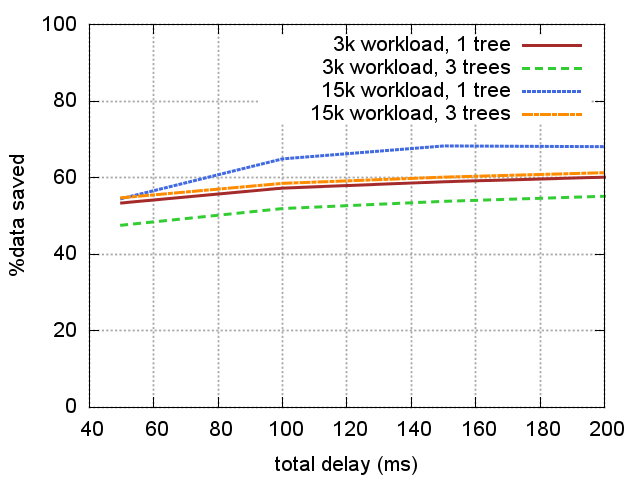
\includegraphics[width=3in]{img/savings.png}
\end{center}
\caption{\label{fig:savings} Effect of changing total message delay on
bandwidth savings.}
\end{figure}

We also evaluate the \emph{effective throughput} of aggregation with data
compaction for the same set of experiments.  The \emph{effective throughput} is
defined as total throughput including messages that are not forwarded due to
data compaction.  Figure~\ref{fig:eff-tp} shows the results. 

The two workload are chosen such that without data compaction, all the messages
generated by the lighter workload could fit into the $1$Gbps bandwith, whereas
the heavier workload well exceeds this bandwidth.  We see that regardless of
whether multiple trees are enabled, the effective throughput of the lighter
workload are almost identical, and they stayed flat with respect to changing
message delays.  This is because virtually all the messages can get through the
system, dispite the actually saving numbers differ, as shown in
Figure~\ref{fig:savings}.  The small difference between the two curves is
caused by queueing overhead.

The two curves of the heavier workload reflectsthe effect of data compaction.
It is not enough to get all the messages through the system using only one
tree.  Therefore, the effective throughput goes up as more delay is injected.
On the other hand, there is enough bandwidth with the help of three trees, and
all the messages can get through the system.

\begin{figure}[t]
\begin{center}
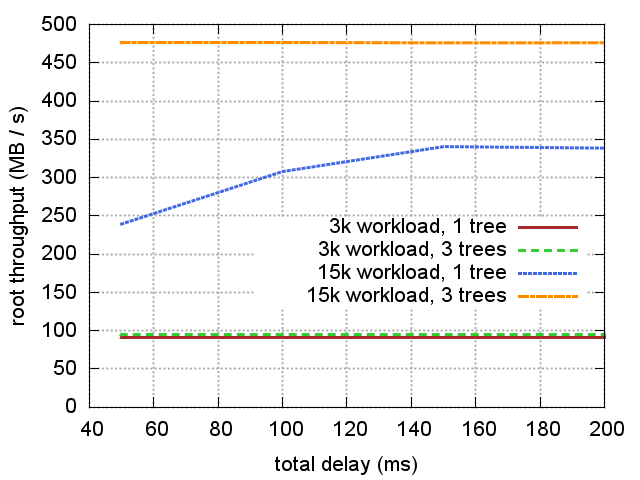
\includegraphics[width=3in]{img/eff-tp.png}
\end{center}
\caption{\label{fig:eff-tp} Effect of changing total message delay on
effective throughput.}
\end{figure}

\subsection{Message Delay Distribution}

This experiment takes a closer look at bandwidth saving from individual nodes,
and the effect of changing the policy of distributing message delay among
nodes.  We used the heavier workload described previously with only one tree.
Data compaction is enabled.  The total message delay is fixed at $100$ms.
Other experiment setup are the same as in the last section.

We include three policies of message delays.  Case $1$ divides the $100$ms
delay uniformly across all the levels in the tree; case $2$ and $3$ distributes
the delay proportionally across tree levels.  In case $2$, the closer a node to
root, the longer delay it gets; case $3$ is the opposite.

\begin{figure}[t]
\begin{center}
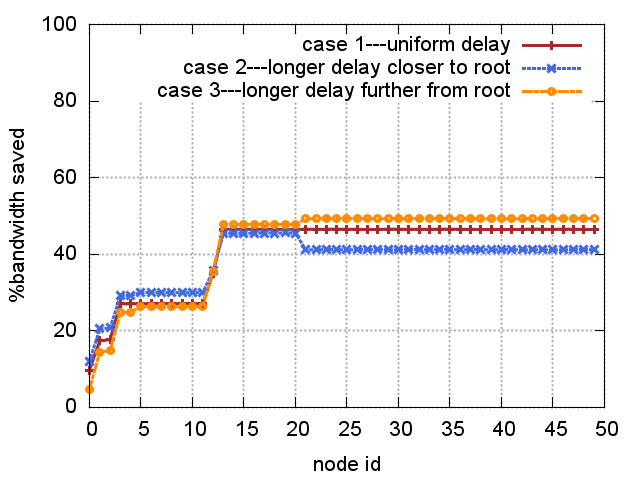
\includegraphics[width=3in]{img/node_saving.png}
\end{center}
\caption{\label{fig:node-saving} Outbound bandwidth of each node with data compaction
enabled.  Nodes are sorted in decreasing bandwidth utilization.}
\end{figure}

Figure~\ref{fig:node-saving} shows the result of bandwidth saving at each
individual node.  Nodes are sorted by the level-order traversal of the tree.
At each particular node, longer delay results in more saving of bandwidth.  In
all cases, the first three levels of the nodes show much less saving
percentages than the leaves.

\begin{table}[h]
\begin{center}
\begin{tabular}{|c|c|c|c|}
\hline
 & Case 1 & Case 2 & Case 3 \\ \hline
Savings & 64.89\% & 67.32\% & 60.97\% \\ \hline
\end{tabular}
\end{center}
\caption{\label{tab:saving} Aggregated bandwidth saving with various message
delay distributions.}
\end{table}

Table~\ref{tab:saving} shows the aggregated saving from all nodes for each
case.  Case $2$ has the most savings, suggesting the overall saving numbers are
driven by those nodes closer to the root, which operate on larger amount of
data collected from their entire subtrees.


\subsection{Load Balancing with Multiple Trees}

One of the goals of having multiple trees is to reduce load imbalance across
the nodes.  To evaluate the effect of using multiple trees on load balancing,
we investigate the bandwidth utilization by each node under various setup.

Figure~\ref{fig:bw-gc} shows a breakdown of outbound bandwidth usage at all the
nodes.  We used the same workload described in the last section.

With alternative path enabled by multiple trees, loads are distributed more
evenly across nodes.  Although the three root node nodes still carry much
higher loads, they are further from saturating the links.

\begin{figure}[t]
\begin{center}
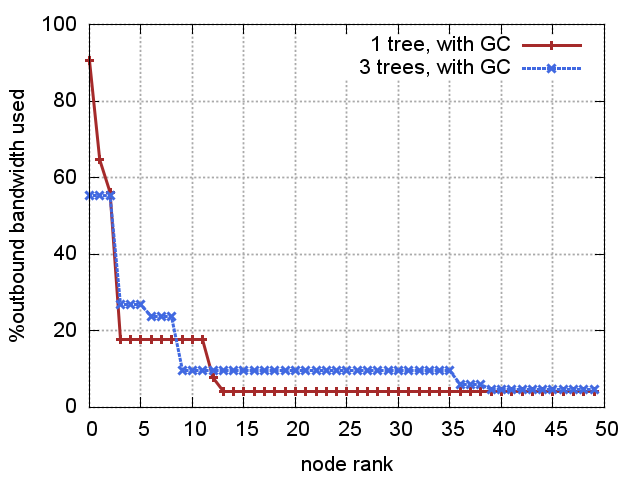
\includegraphics[width=3in]{img/bw-gc.png}
\end{center}
\caption{\label{fig:bw-gc} Outbound bandwidth of each node with data compaction
enabled.  Nodes are sorted in decreasing bandwidth utilization.}
\end{figure}

\begin{figure}[t]
\begin{center}
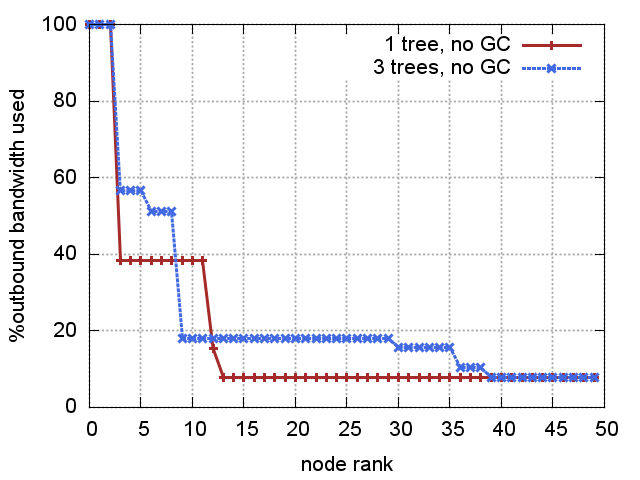
\includegraphics[width=3in]{img/bw-nogc.png}
\end{center}
\caption{\label{fig:bw-nogc} Outbound bandwidth of each node with data
compaction enabled.  Nodes are sorted in decreasing bandwidth utilization.}
\end{figure}

Figure~\ref{fig:bw-nogc} shows the breakdown of outbound bandwidth usage of the
same experiments, but with data compaction disabled.  Without data compaction,
the system cannot handle the large amount of messages generated.  Even with
multiple trees, all the root nodes are being completely saturated.  However,
the use of multiple trees makes extra bandwidth available, and the total amount
of messages sent through the system (represented by the area under each curve,
since no message is discarded) still gets higher.


\section{Related Work}\label{sec:related}

The data aggregation problem addressed in this paper shares many
characteristics with multicast systems.  In fact, many existing
application-level multicast systems either build overlay trees, or rely on such
structures implicitly to disseminate data.  Examples include
Overcast~\cite{JGJK00}, Chainsaw~\cite{PKTSM05}, SelectCast~\cite{BvRD03}, and
Bayeux~\cite{ZZJKK01}.  The main difference is that with multiple publisher
and a single receiver, the data aggregation system has the ability to perform
data compaction to improve bandwidth efficiency within the tree structures.
Our system also provide adaptive bandwidth allocation to accomodate many data
sources behaving differently.

SplitStream~\cite{CDKNRS03} is a multicast system that uses multiple
independent trees to achieve efficiency and fault tolerance.  SplitStream built
multicast trees based on Pastry, an underlying peer-to-peer overlay
network~\cite{RD01}, while our design builds aggregation trees based on
knowledge of the underlying physical network topology.

Astrolabe~\cite{vRBV03} is a scalable distributed service that supports data
aggregation.  It works by organizing resources into a hierarchy of domains.
Astrolabe provides the ability of querying aggregated data using a high-level
language.  However, it is not intended for an environment in which a large
number of nodes proactively push updates to one destination at high rate.

The data compaction technique is related to the garbage collection mechanism
introduced in Sprinkler~\cite{GvR13}.  Garbage collection in Sprinkler operates
on a sequence of events with total order.  We generalize the concept and make
use of it on an unordered set of messages.  Also, Sprinkler scales with a large
number of subscribers in geo-distributed datacenters, but it doesn't scale with
the number of publishers.

QJUMP~\cite{QJUMP15} is a system that offers priority levels with different
tradeoffs between latency variance and throughput.  Our system aims at reducing
loac imbalance, and trades off latency for saving on bandwidth.


\section{Conclusion}\label{sec:conclusion}

This paper presents the design of a scalable overlay facility for data
aggregation in datacenter network environment.  Our design achieves scalability
across a large number of nodes through the use of multiple independent
aggregation trees and efficient data compaction.  The system is adaptive to
heterogeneous data sources, and is resilient to failures.  An initial
simulation study shows encouraging performance results, and helps us understand
the characteristics of the system.


%\acks
%Acknowledgments, if needed.

% We recommend abbrvnat bibliography style.

\newpage
\bibliographystyle{abbrvnat}
\bibliography{references}

% The bibliography should be embedded for final submission.

%\begin{thebibliography}{}
%\softraggedright

%\bibitem[Smith et~al.(2009)Smith, Jones]{smith02}
%P. Q. Smith, and X. Y. Jones. ...reference text...

%\end{thebibliography}


\end{document}
